\ifdefined\maindoc
\else
\documentclass[12pt]{report}
\usepackage[a4paper,left=40mm,right=25mm,top=25mm,bottom=25mm]{geometry}
\usepackage[utf8]{inputenc}
\usepackage[T1]{fontenc}
\usepackage[british]{babel}
\usepackage{amsmath,amssymb}
\usepackage{booktabs}
\usepackage{setspace}
\usepackage{graphicx}
\usepackage{enumitem}
\usepackage{placeins}
\usepackage{hyperref}
\usepackage[backend=biber,style=ieee,citestyle=numeric-comp,sorting=none]{biblatex}
\addbibresource{../../references.bib}
\onehalfspacing
\graphicspath{{figures/}}
\makeatletter
\newlabel{ch:main-intro}{{1}{1}{}{Doc-Start}{}}
\newlabel{ch:lit-review}{{2}{1}{}{Doc-Start}{}}
\newlabel{ch:system-model}{{3}{1}{}{Doc-Start}{}}
\newlabel{ch:diamond-module}{{4}{1}{}{Doc-Start}{}}
\newlabel{ch:probability-toolkit}{{5}{1}{}{Doc-Start}{}}
\newlabel{ch:capacity-toolkit}{{6}{1}{}{Doc-Start}{}}
\newlabel{ch:critical-path}{{7}{1}{}{Doc-Start}{}}
\newlabel{ch:julia-package}{{8}{1}{}{Doc-Start}{}}
\newlabel{ch:front-end}{{9}{1}{}{Doc-Start}{}}
\newlabel{ch:conclusions}{{11}{1}{}{Doc-Start}{}}
\newlabel{app:network-specs}{{A}{1}{}{Doc-Start}{}}
\newlabel{app:full-results}{{B}{1}{}{Doc-Start}{}}
\makeatother
\newcommand{\CaseStudyNetwork}{Net3}
\begin{document}
\title{An End-to-End Application: One Network, Three Analyses}
\fi

\providecommand{\PH}[1]{\textbf{[#1]}}

\section{Introduction}
\label{sec:e2e-intro}

Each of Chapters~\ref{ch:probability-toolkit} to~\ref{ch:critical-path} applied its toolkit
to a network of its own. None of them could show the claim of Chapter~\ref{ch:main-intro}
that one model of a system serves all three analyses without the topology being entered
again, because each demonstrated one analysis. This chapter shows it. A single water
distribution network is converted once, uploaded through the interface of
Chapter~\ref{ch:front-end}, and analysed by all three toolkits under several scenarios,
and every number reported here is the one the server returned, with the request and
response recorded beside it.

The network is \CaseStudyNetwork, the third example network distributed with EPANET
\cite{rossman2000epanet2}. Section~\ref{sec:e2e-network} describes how it was oriented and
what the graph object found in it. Section~\ref{sec:e2e-inputs} derives the inputs for the
three interpretations and states which values are from a source and which are assumed.
Sections~\ref{sec:e2e-reliability} to~\ref{sec:e2e-schedule} give the results of each
toolkit, Section~\ref{sec:e2e-profile} places two of them on the same drawing, and
Section~\ref{sec:e2e-findings} records what the run showed about the framework itself:
two boundaries reached and three errors found. Section~\ref{sec:e2e-summary} closes.

\section{The Network}
\label{sec:e2e-network}

\CaseStudyNetwork{} models a water distribution system with two reservoirs, a lake and a
river, three storage tanks, ninety-two junctions, 117 pipes and two pumps. It is
distributed with EPANET as a test case and its input file is public, so the structure has a
citable source and the conversion can be repeated. The file used is the copy bundled with
WNTR 1.5.0; its hash is recorded in Appendix~\ref{app:network-specs}.

The physical network is meshed, and the model of Chapter~\ref{ch:system-model} requires an
acyclic graph, so each link was oriented by the direction of its flow in a hydraulic
simulation. The simulation is the input file's own seven-day run, and the orientation is
taken at its final time step. Every link received a direction from the sign of its flow;
three links carried zero flow at that step and kept the direction the file declares. No
link had to be dropped or merged: the flow-oriented network was already acyclic. This is
the operating-snapshot assumption of Chapter~\ref{ch:system-model} applied to a real
system, and it holds here without adjustment.

The graph object built from the oriented edge list has 97 nodes and 119 edges. Its sources
are the two reservoirs and one tank that the simulation shows discharging at the chosen
step; its eighteen sinks are sixteen demand junctions and the two tanks that are filling.
There are 35 forks, 23 joins and 28 layers. The decomposition of
Chapter~\ref{ch:diamond-module} finds 21 maximal diamonds and 307 unique diamonds including
nested ones, with a maximum conditioning width of 12 (Figure~\ref{fig:e2e-network}). An earlier conversion of the same file was oriented by breadth-first search from a
chosen root, as the metro network of Chapter~\ref{ch:probability-toolkit} was. It has
almost the same number of maximal diamonds and a width of 5. The hydraulic orientation
keeps more of the network's real loop structure, and the deeper nesting follows from it.

\begin{figure}[htbp]
  \centering
  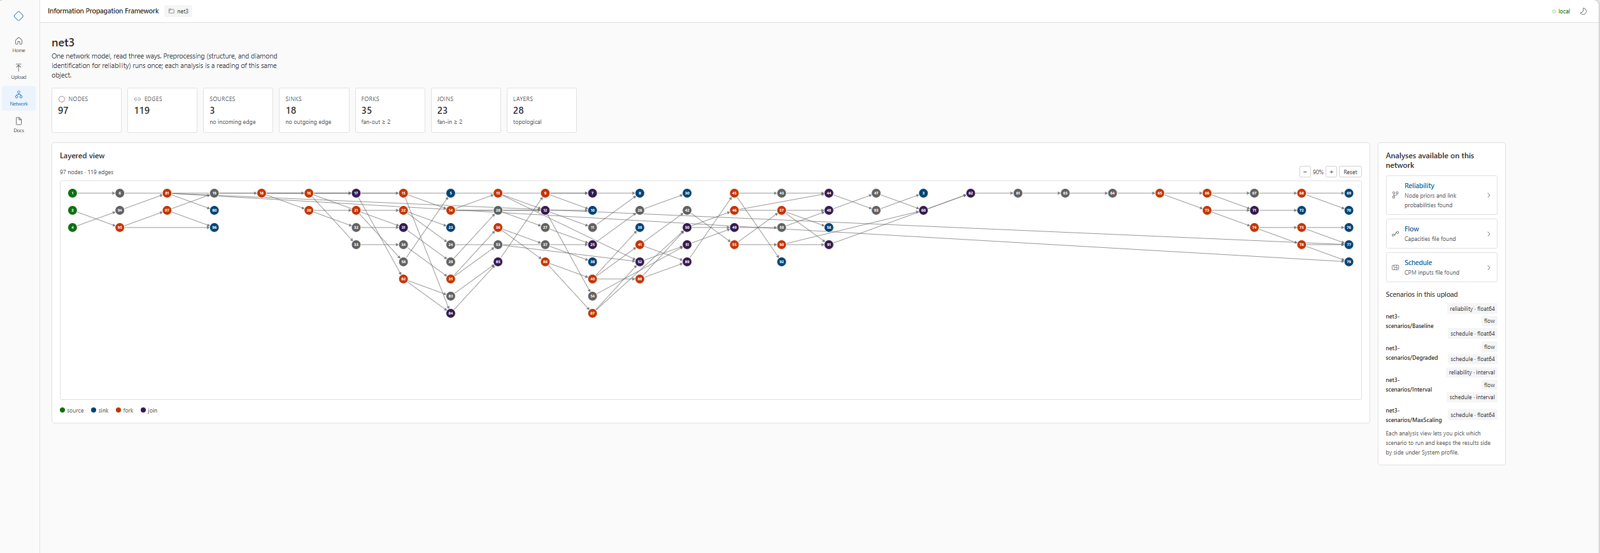
\includegraphics[width=\linewidth]{fig01_network.png}
  \caption{The network page after upload: 97 nodes, 119 edges, 3 sources, 18 sinks, 35 forks,
  23 joins and 28 layers, with the four scenario folders and the analyses each supports.}
  \label{fig:e2e-network}
\end{figure}

\section{Inputs}
\label{sec:e2e-inputs}

Four scenario folders were uploaded with the structure file. The capacity analysis reads its
own copy of the structure file, with a super-sink added, for the reason given under the
capacity inputs below. Every value below is either
taken from a source, computed from the input file, or assumed and named as such.

\subsection{Reliability inputs}

Every node prior is exactly one. A junction is a demand point, and the reservoirs and tanks have no failure mode in this
model, so reliability lives on the edges.
The two pumps carry 0.99, the level the pumping literature treats as appropriate for a
critical asset where failure between overhauls is not acceptable \cite{butts2022pumpreliability};
this is general guidance; no figure exists for these pumps. Three links are placeholder
tank connectors in the input file, with a length of 99 feet, a diameter of 99 inches and a
roughness of 199, and they carry exactly one. The remaining 114 pipes carry the probability of no break in one year under an annual
break-rate model. The rates are breaks per hundred mile-years by diameter class from the
Utah State University survey of North American mains \cite{barfuss2023breakrates}: 13.3
for 3 to 12 inches, 3.1 for 14 to 24 inches and 0.2 for 30 to 36 inches, all materials
combined since the file records no material. The rate times the pipe length gives the
expected number of breaks, and the Poisson probability of none is the edge value. The resulting pipe probabilities range from 0.891, on the longest
small-diameter main, to 1.000. An interval scenario widens every value that is not exactly
one by five per cent either side.

A probability-box scenario was not run. The sum over the 307 diamonds of $2^{|C|}$ is
$5.5 \times 10^{4}$, beyond the point at which a comparably costed drone design in
Chapter~\ref{ch:probability-toolkit} did not complete within its budget, and the
tractability boundary of the probability-box form is characterised in that chapter.

\subsection{Capacity inputs}

Capacities are in litres per second throughout. Each pipe's capacity is the flow at a
velocity of 1.5 metres per second through its stated diameter, the conservative end of the
range in Section~\ref{sec:e2e-inputs}'s convention; each pump's is the largest flow point of
its own curve in the input file, 252.4 for the lake pump and 883.3 for the river pump; the
reservoir edges and the three placeholder connectors are unbounded. To measure throughput
against demand, the construction of Chapter~\ref{ch:capacity-toolkit}'s IEEE case is used:
a super-sink with one edge from each of the 58 demand junctions, capacity equal to that
junction's demand at the simulation step, 680.1 litres per second in total. The super-sink
and its 58 edges are added to the edge list the capacity analysis reads, which then has 98
nodes and 177 edges, and the capacity file names the super-sink as the only sink. Without
that declaration the two filling tanks and the one dead-end junction without demand would
also count as delivery points. A degraded scenario derates the network's
dominant transmission main, an 8.6-mile 30-inch pipe that is by a wide margin the longest
large-diameter link, to half its capacity, and takes the river pump, the larger of the two,
out of service.

\subsection{Schedule inputs}

The schedule interpretation is a restoration programme: the recommissioning of every pipe,
pump and tank after a shutdown, in the order the network's dependencies impose. Durations
follow the procedure a North American utility specifies for new and repaired mains
\cite{awwa2017c600,awwa2017c605,awwa2014c651}: one hour to isolate (assumed), a two-hour
pressure test, a flush of three pipe volumes at three feet per second, a 24-hour
chlorination hold and 40 hours of bacteriological sampling. Every pipe therefore carries 67
hours plus its flush time, which ranges from minutes to 12.6 hours on the trunk main. The
two regulatory holds dominate every pipe's duration; this is how restoration is in practice, gated by
disinfection procedure. Pumps carry eight hours and tanks
24, both assumed, since the standards cover neither. Reservoirs and junctions carry zero.
An interval scenario widens every duration by twenty per cent either side. A fourth
scenario carries the reliability edge probabilities as multiplicative factors with unit
node values, for the MaxScaling mode of Chapter~\ref{ch:critical-path}.

\section{Reliability}
\label{sec:e2e-reliability}

Under the deterministic inputs, the belief that supply reaches a node ranges from 0.806 at
node 76 to 1 at the sources, with a mean of 0.934 over the network and 0.928 over the
eighteen sinks (Figure~\ref{fig:e2e-belief}). The lowest values sit at the far end of the
long small-diameter mains, where the product of many pipe probabilities accumulates and
no second route compensates. The five nodes reported in Appendix~\ref{app:full-results}
as a spot check, 32, 29, 81, 54 and 78, carry 0.856, 0.930, 0.977, 0.810 and 0.843. The
propagation took 4.6 seconds in a warm process; identification was reused from the store
after its first computation.

\begin{figure}[htbp]
  \centering
  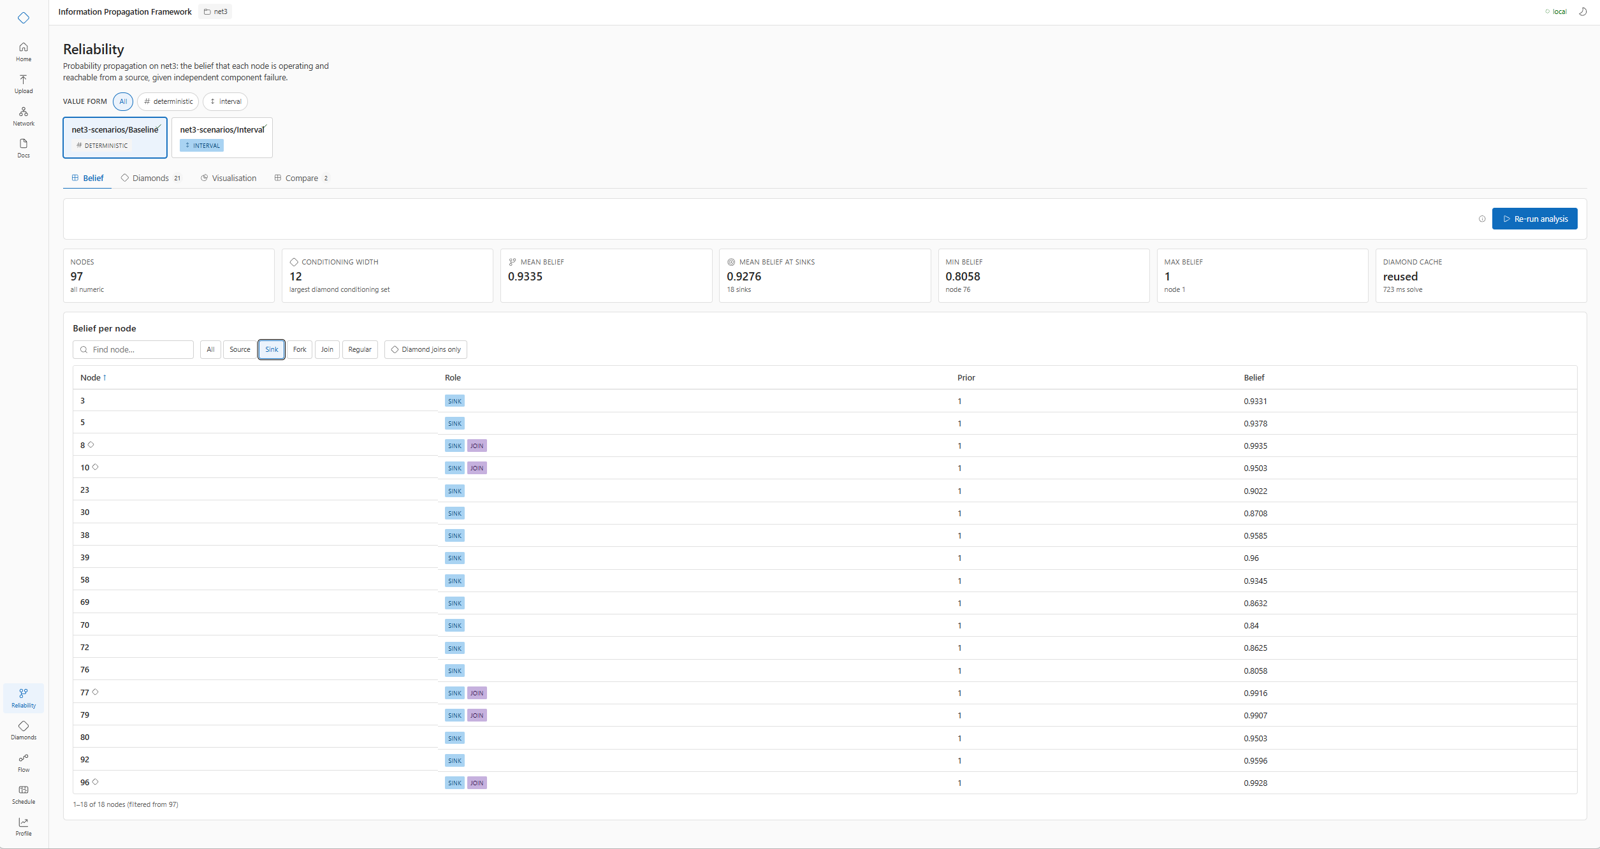
\includegraphics[width=\linewidth]{fig02_belief_baseline.png}
  \caption{Reliability, deterministic scenario, filtered to the eighteen sinks: the belief
  at each, with the summary tiles above. Conditioning width 12; minimum belief 0.806 at
  node 76.}
  \label{fig:e2e-belief}
\end{figure}

Under the interval inputs the picture changes (Figure~\ref{fig:e2e-belief-interval}). A five per cent widening on each
pipe produces a mean band of 0.36 across the network and a maximum of 0.64 at node 76,
whose belief lies in $[0.354, 0.990]$. The widening compounds along the same long chains
that lowered the point beliefs, and the 307 diamonds mean that an interval on one pipe
enters many nodes' ranges through several routes. The upper bounds stay near one at most
sinks, because the corner in which every pipe is at its upper probability is a highly
reliable network; the lower bounds fall sharply, because the opposite corner is not. A
point analysis at the central values reports 0.934; the exact range says that the same
network, under uncertainty a utility would regard as modest, cannot be certified above
0.35 at its worst-served junction. Which of the two a planner should act on is the question
Chapter~\ref{ch:probability-toolkit} posed on the drone network, and this is its answer on
a real one.

\begin{figure}[htbp]
  \centering
  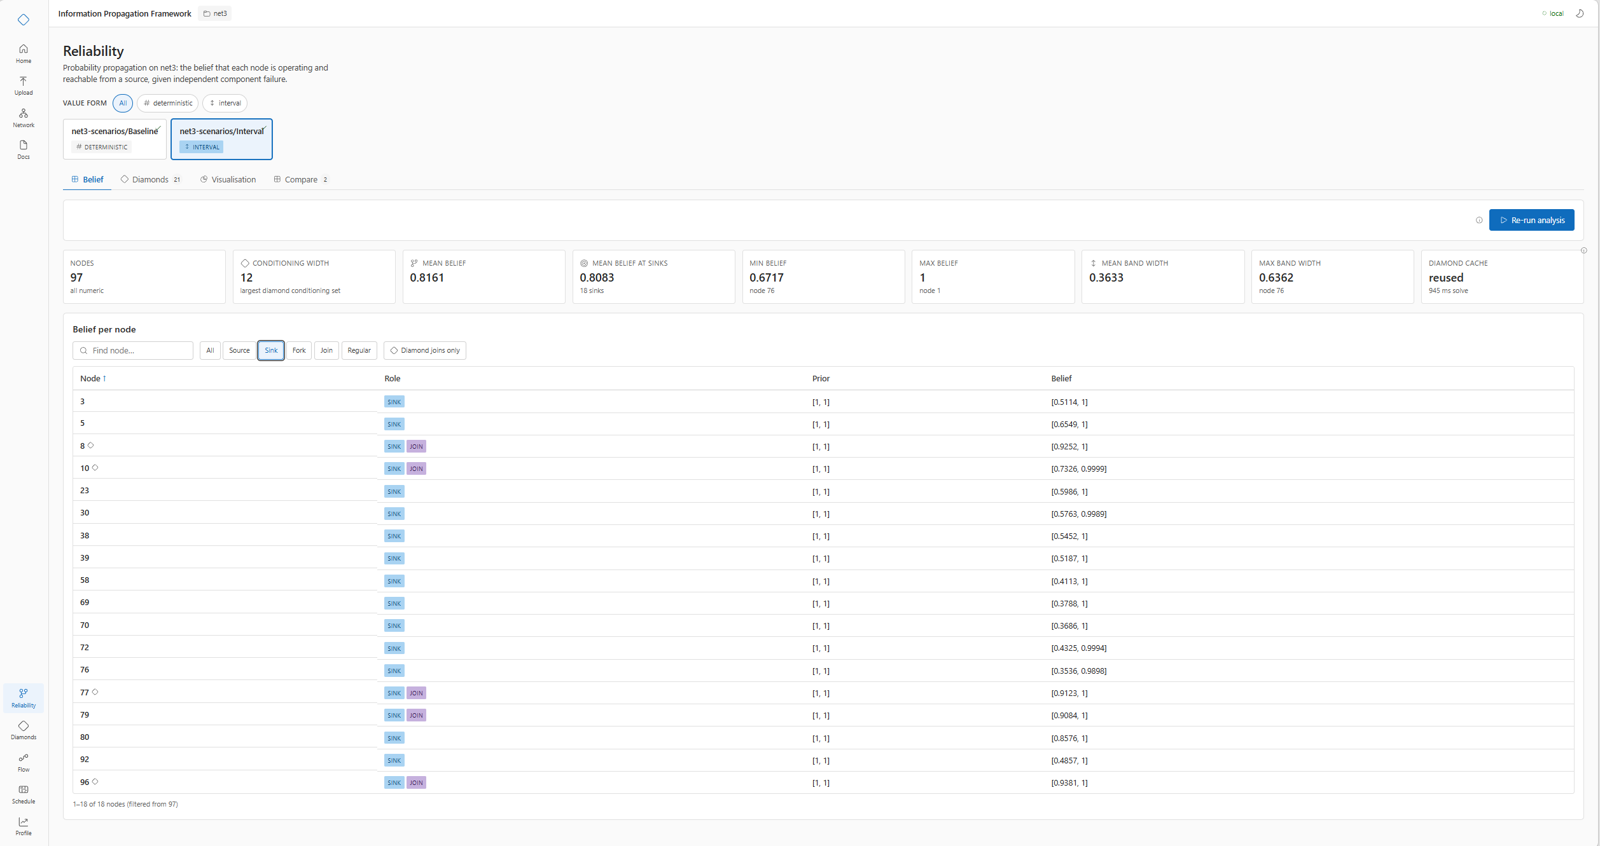
\includegraphics[width=\linewidth]{fig03_belief_interval.png}
  \caption{Reliability, interval scenario, the same eighteen sinks: each belief as a range.
  Mean band 0.363, maximum band 0.636 at node 76.}
  \label{fig:e2e-belief-interval}
\end{figure}

The Diamonds tab (Figure~\ref{fig:e2e-diamonds}) lists the 21 maximal diamonds with their
conditioning sets and nesting. The largest, at join 77, spans 46 nodes and 56 edges and
holds eleven sub-diamonds (Figure~\ref{fig:e2e-diamond77}); the width-12 conditioning set
of the summary tile belongs to a diamond nested inside it, which the detail view reaches
through its sub-diamond list. Every one of the 21 conditions on node 95 alone at its own
level, which is the junction immediately downstream of the river pump: the whole network's
reconvergence is anchored on the point where the two supplies first meet.

\begin{figure}[htbp]
  \centering
  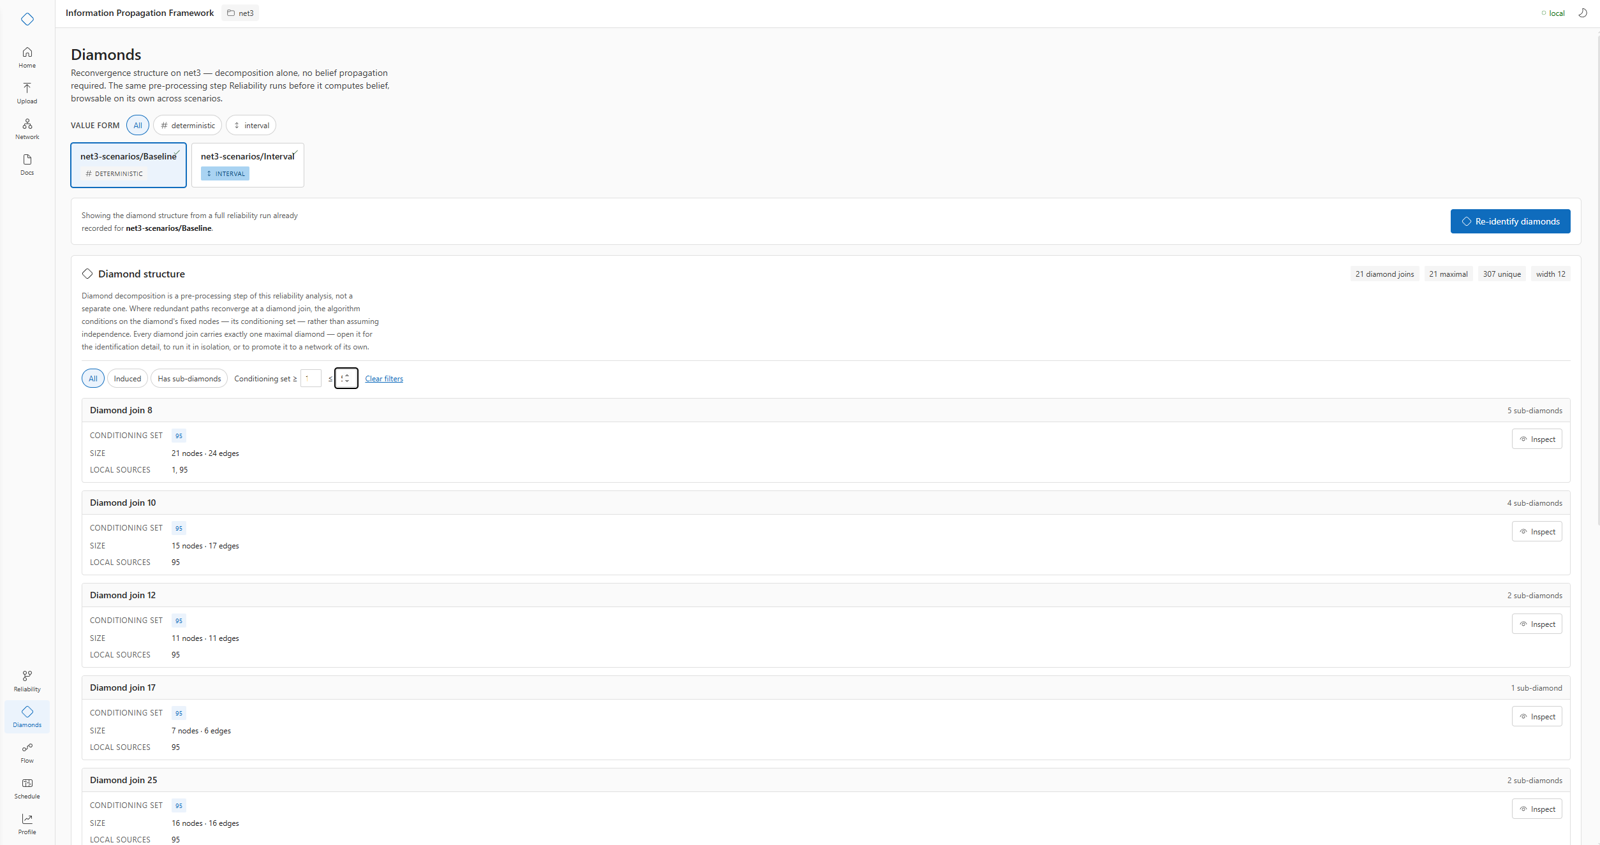
\includegraphics[width=\linewidth]{fig04_diamonds.png}
  \caption{The Diamonds tab: 21 maximal diamonds, 307 unique, width 12. Each entry gives
  the conditioning set, size and local sources, and the number of nested sub-diamonds.}
  \label{fig:e2e-diamonds}
\end{figure}

\begin{figure}[htbp]
  \centering
  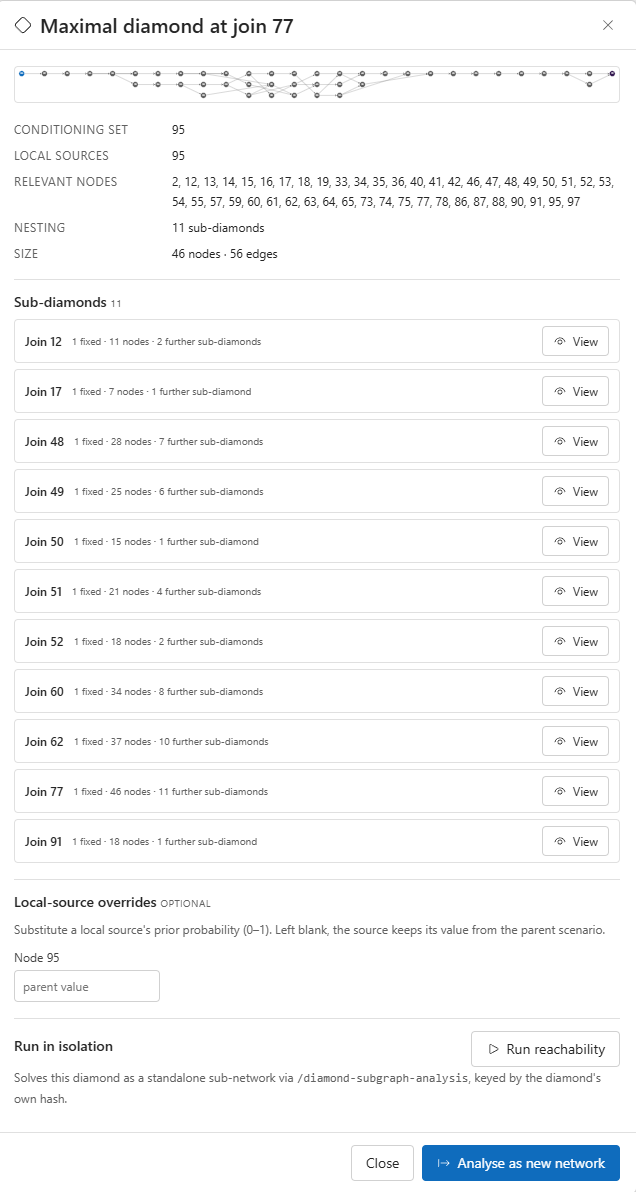
\includegraphics[width=0.5\linewidth]{fig05_diamond_77.png}
  \caption{The detail view of the diamond at join 77: 46 nodes, 56 edges, conditioning
  set $\{95\}$, eleven sub-diamonds, and the controls to run it in isolation or promote it.}
  \label{fig:e2e-diamond77}
\end{figure}

\section{Capacity}
\label{sec:e2e-flow}

The network delivers 680.1 litres per second, the whole demand of the 58 junctions at the
simulation step (Figure~\ref{fig:e2e-flow}). The minimum cut is unique, since the free zone
is empty and the enumeration is complete, and it consists of the 58 demand edges into the
super-sink. Hence the network does not limit delivery at this demand. Two pipes, 18 to 17
and 86 to 87, run full, but neither lies in a minimum cut, so neither bounds the
throughput. There are 401 source-to-sink paths, and no node is a structural single point
of failure. The bottleneck ranking (Figure~\ref{fig:e2e-bottlenecks}) lists the cut edges
from the tightest, the 0.07 litres per second of junction 64, upwards, all at full
utilisation.

\begin{figure}[htbp]
  \centering
  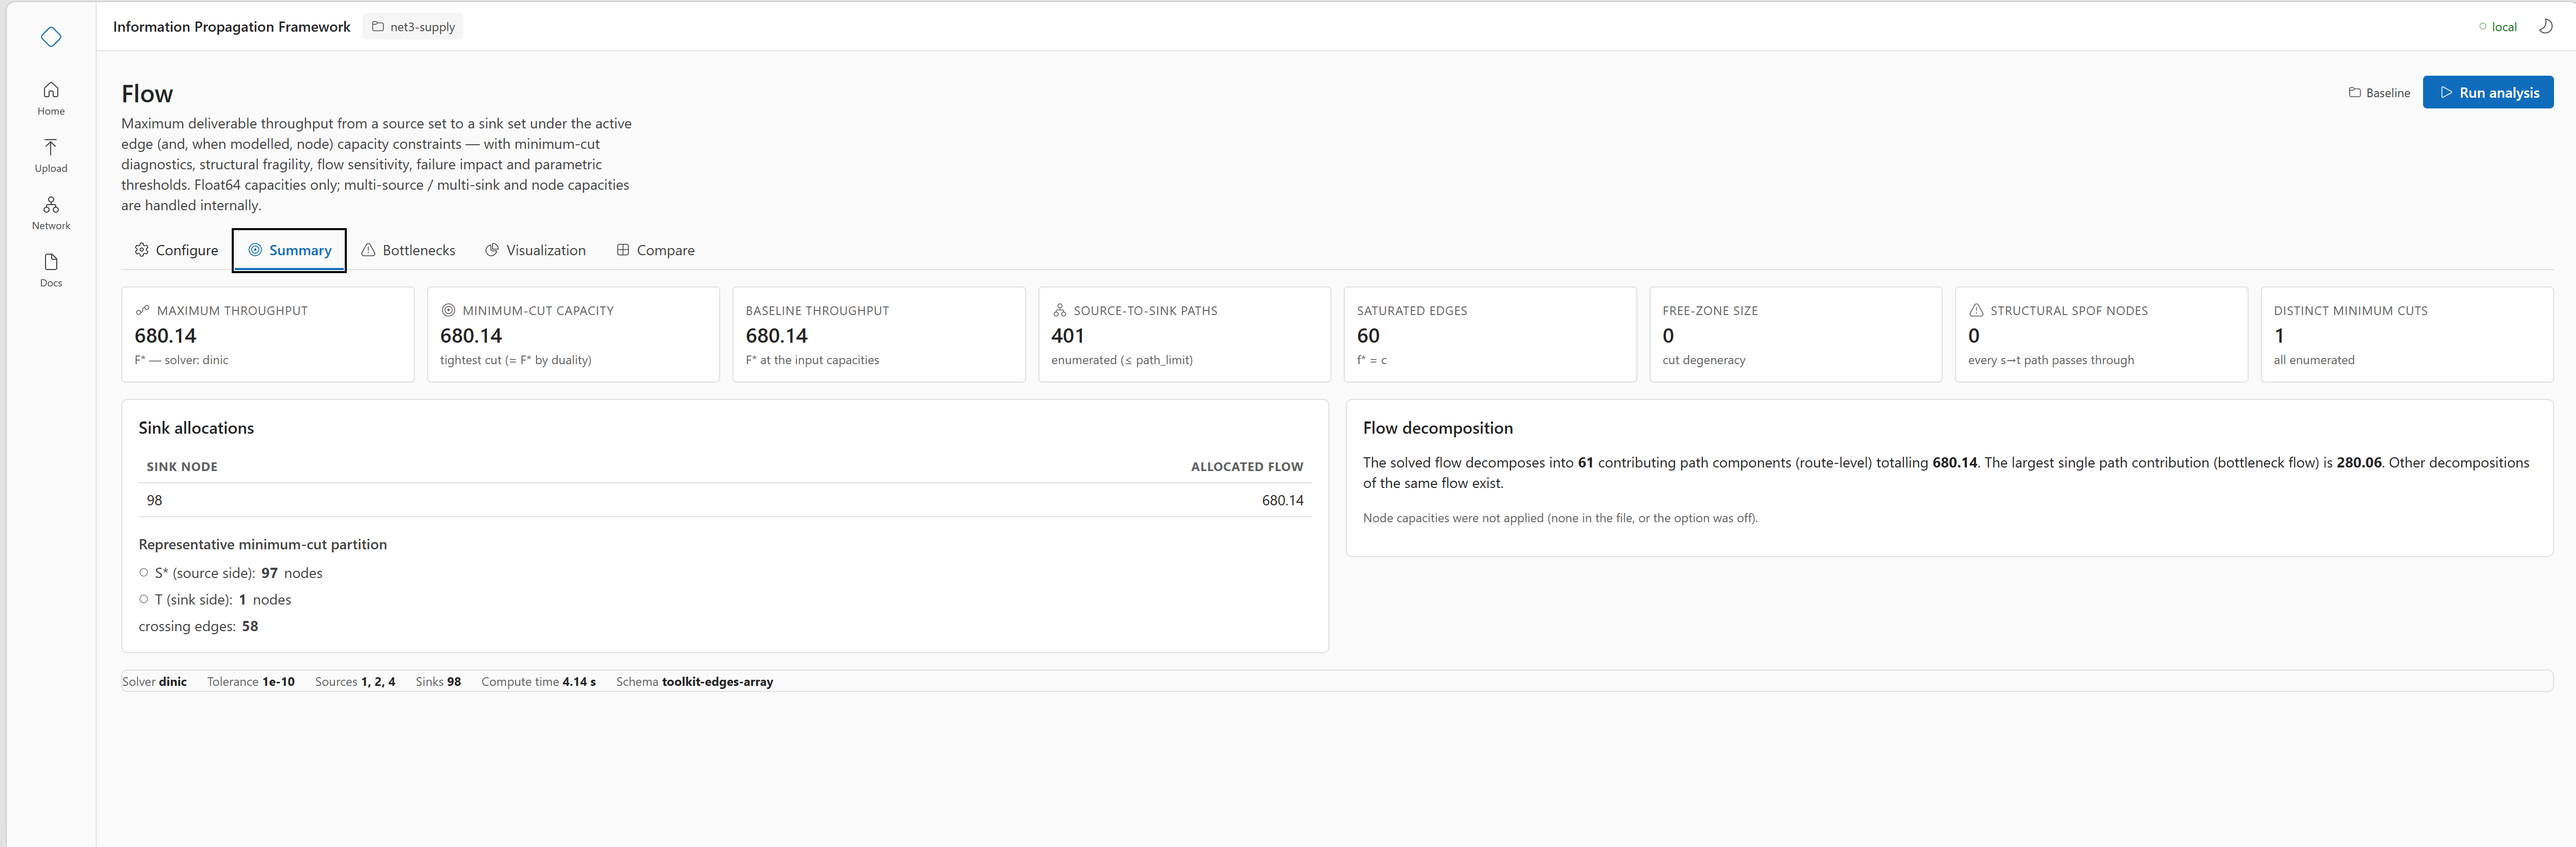
\includegraphics[width=\linewidth]{fig06_flow_baseline.png}
  \caption{Flow summary, baseline: throughput 680.1 litres per second, equal to the total
  demand, with a unique minimum cut of the 58 demand edges, 401 source-to-sink paths and no
  structural single point of failure.}
  \label{fig:e2e-flow}
\end{figure}

\begin{figure}[htbp]
  \centering
  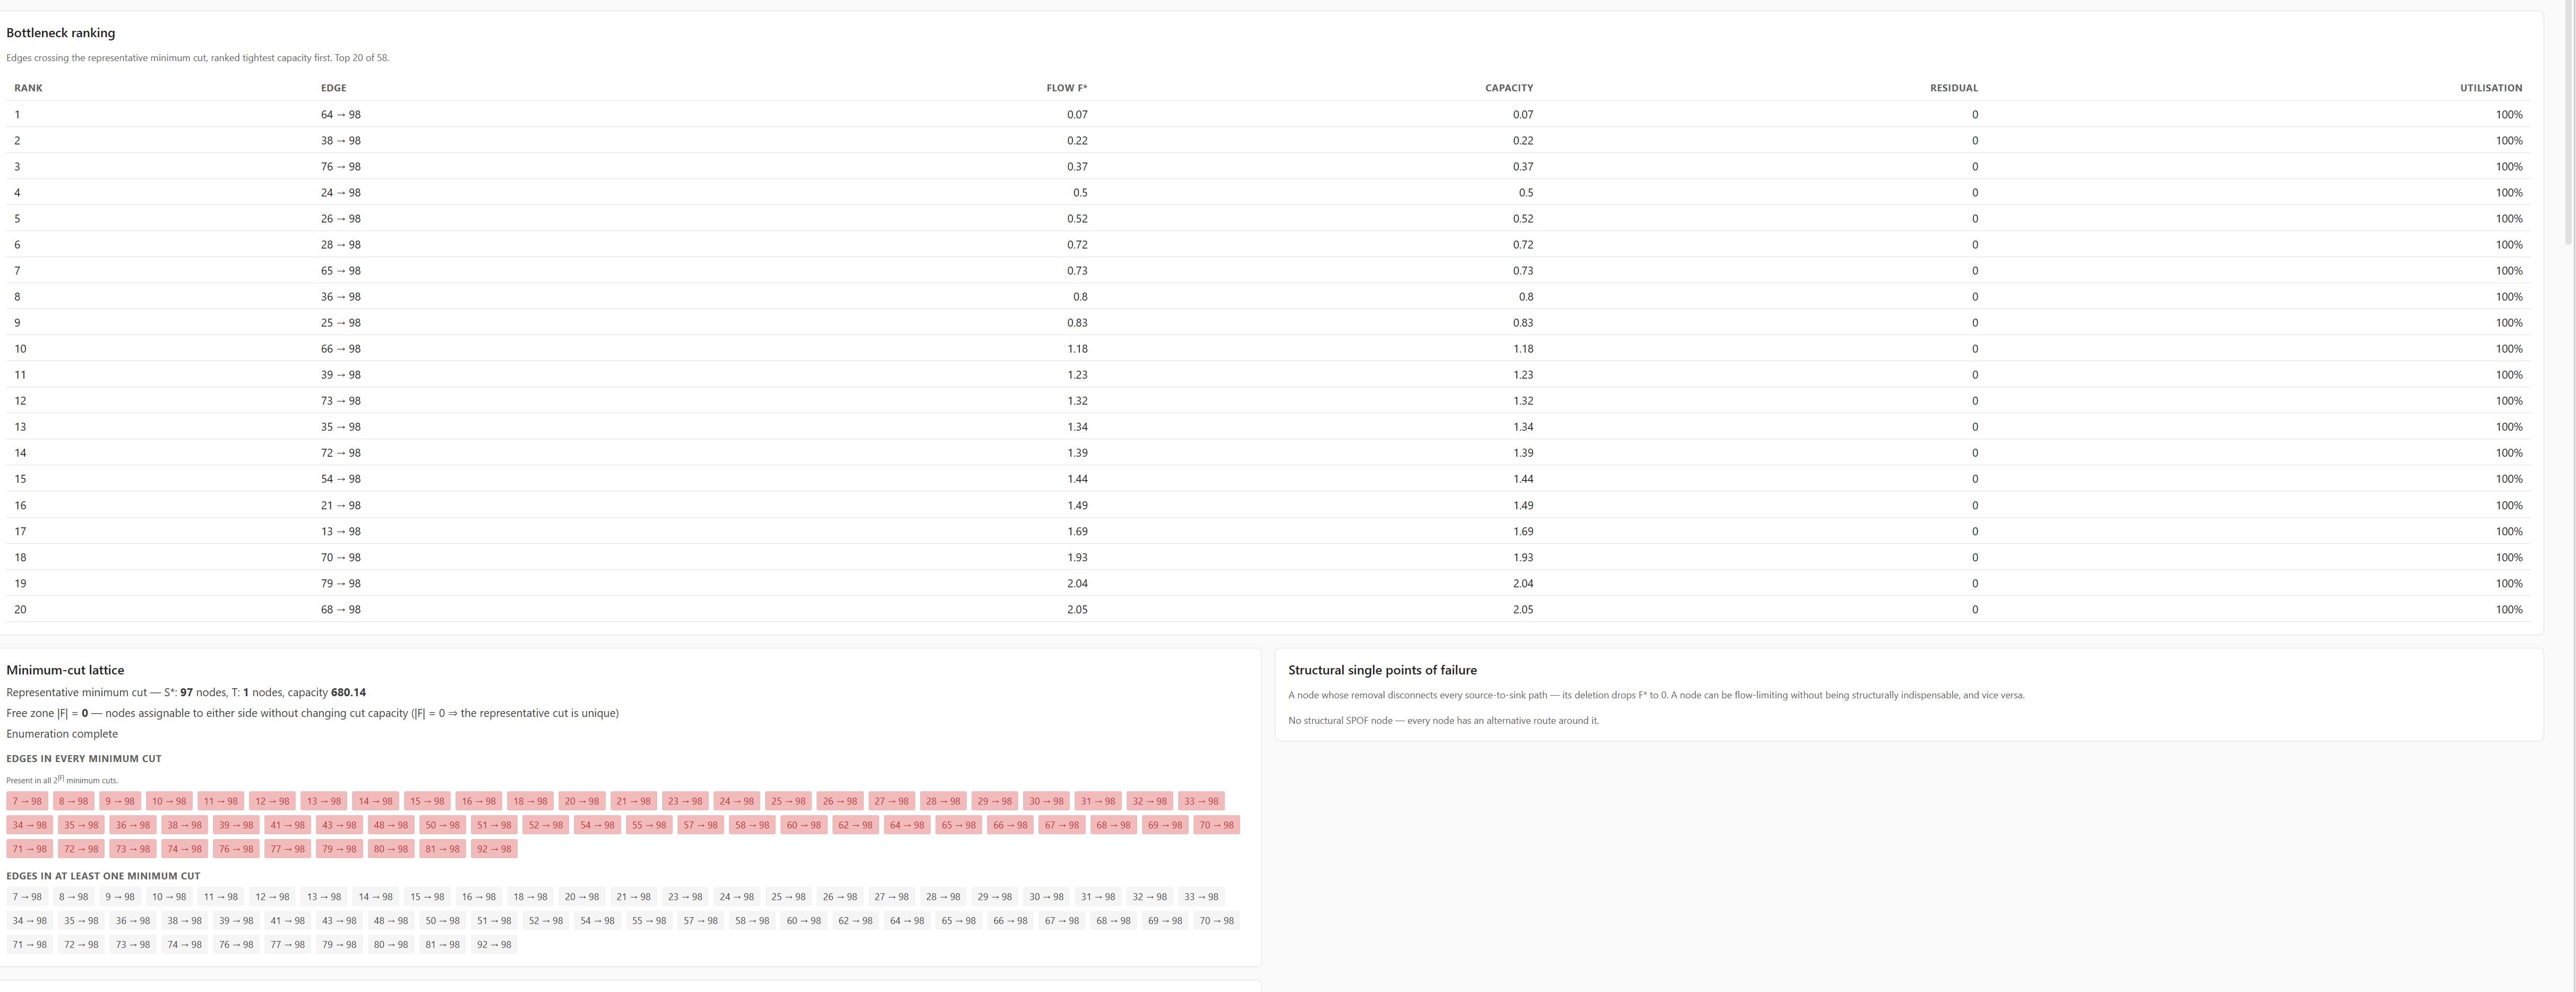
\includegraphics[width=\linewidth]{fig08_flow_bottlenecks.png}
  \caption{Flow bottlenecks, baseline: the edges of the minimum cut ranked by capacity, the
  lattice with its empty free zone and the 58 edges in every minimum cut, and the panel of
  structural single points of failure, which is empty.}
  \label{fig:e2e-bottlenecks}
\end{figure}

Because the cut is the demand, the sensitivity table (Figure~\ref{fig:e2e-sensitivity})
ranks the junctions by their demand. Removing the demand edge of junction 58 loses 280.1
litres per second, and that of junction 92 loses 103.3. Each unit of capacity added to a
demand edge adds one unit of throughput, and the marginal ranges are finite, 327.3 for
junction 58. Every demand edge is critical in the single-failure table, since its loss is
the loss of that junction's demand, and the worst pair is junctions 58 and 92 together, at
383.3 litres per second.

Under the degraded scenario the throughput falls to 43.3 litres per second, 6.4 per cent of
demand (Figure~\ref{fig:e2e-degraded}). Unlike the baseline, the cut is no longer unique.
Enumeration finds 24 minimum cuts over a free
zone of six nodes, and seven edges lie in every one of them: the river pump, now at zero
capacity, and the demand edges of junctions 7, 8, 77, 79, 80 and 81. Those six junctions
are fully served and the other 52 receive less than their demand. In the oriented graph,
junctions 7 and 8 lie downstream of the lake pump and junctions 77 to 81 downstream of the
discharging tank, and no other junction can be reached from either source. The derated
trunk main does not bind, because the river pump is its only feed. It is therefore the
throughput of the network with every pipe held in its snapshot direction. In the
physical network the lake pump could drive water through pipes that ran the other way at
the snapshot, which the oriented model cannot represent. This is a limitation of the
operating-snapshot assumption of Chapter~\ref{ch:system-model}, and a degraded state needs
an orientation of its own.

\begin{figure}[htbp]
  \centering
  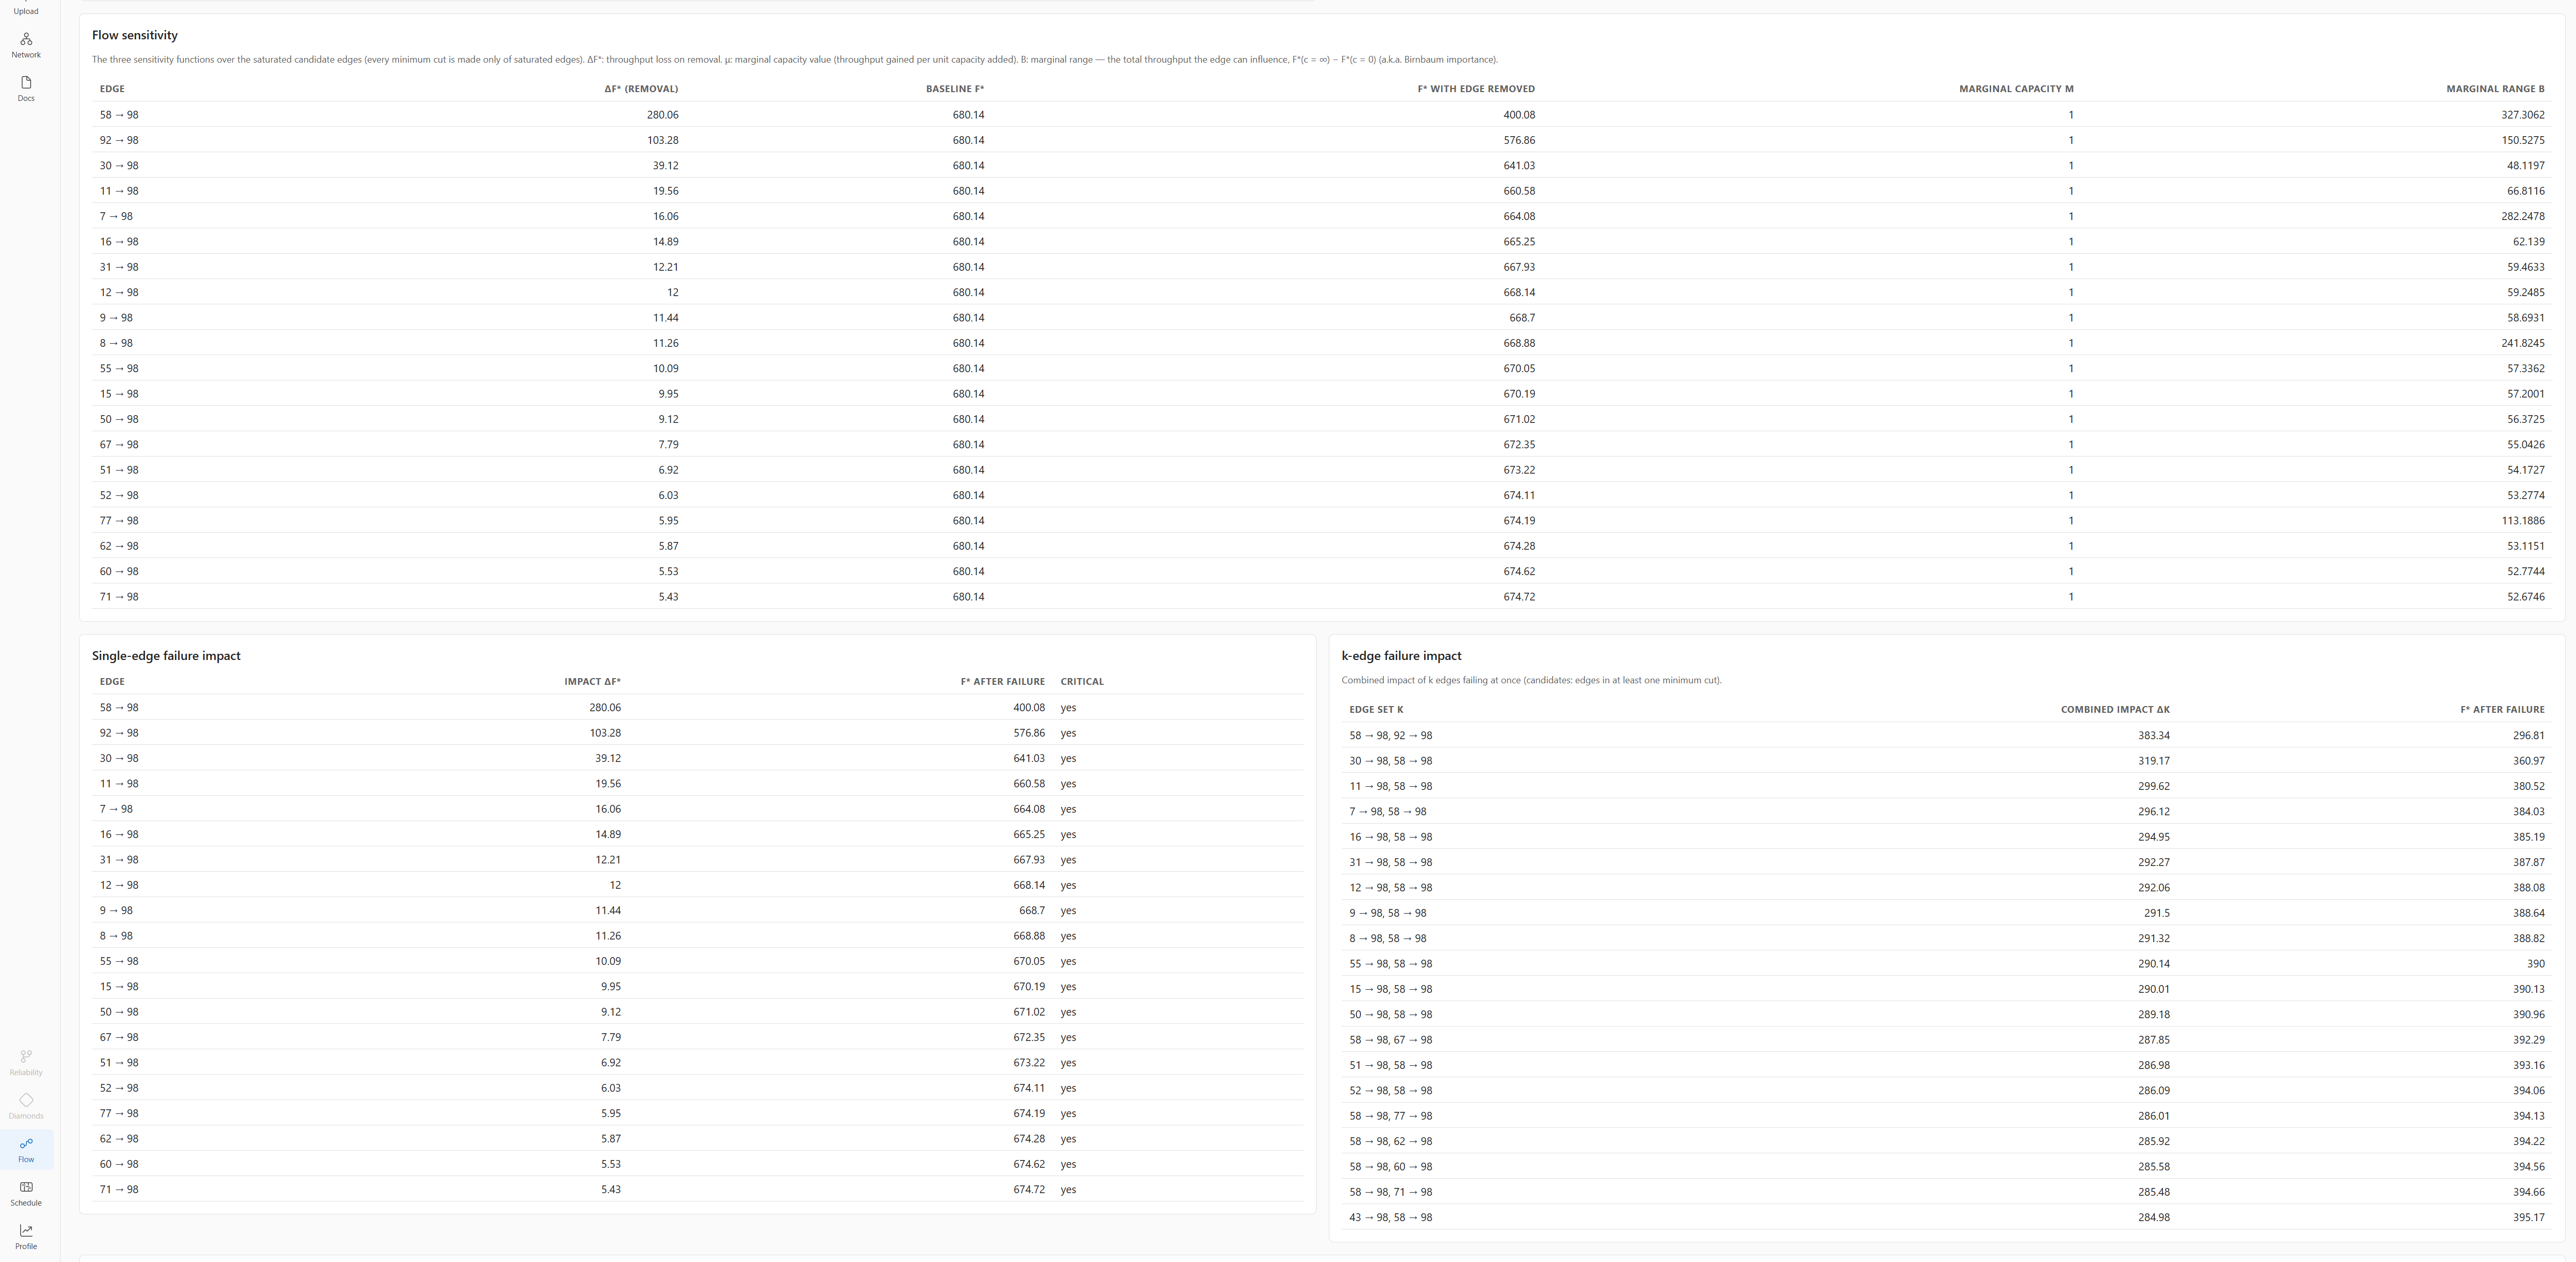
\includegraphics[width=\linewidth]{fig07_flow_sensitivity.png}
  \caption{Flow sensitivity and failure impact, baseline. The sensitivity and single-edge
  tables rank the demand edges by the junction's demand; the $k$-edge table gives the
  combined loss of each pair of cut edges.}
  \label{fig:e2e-sensitivity}
\end{figure}

\begin{figure}[htbp]
  \centering
  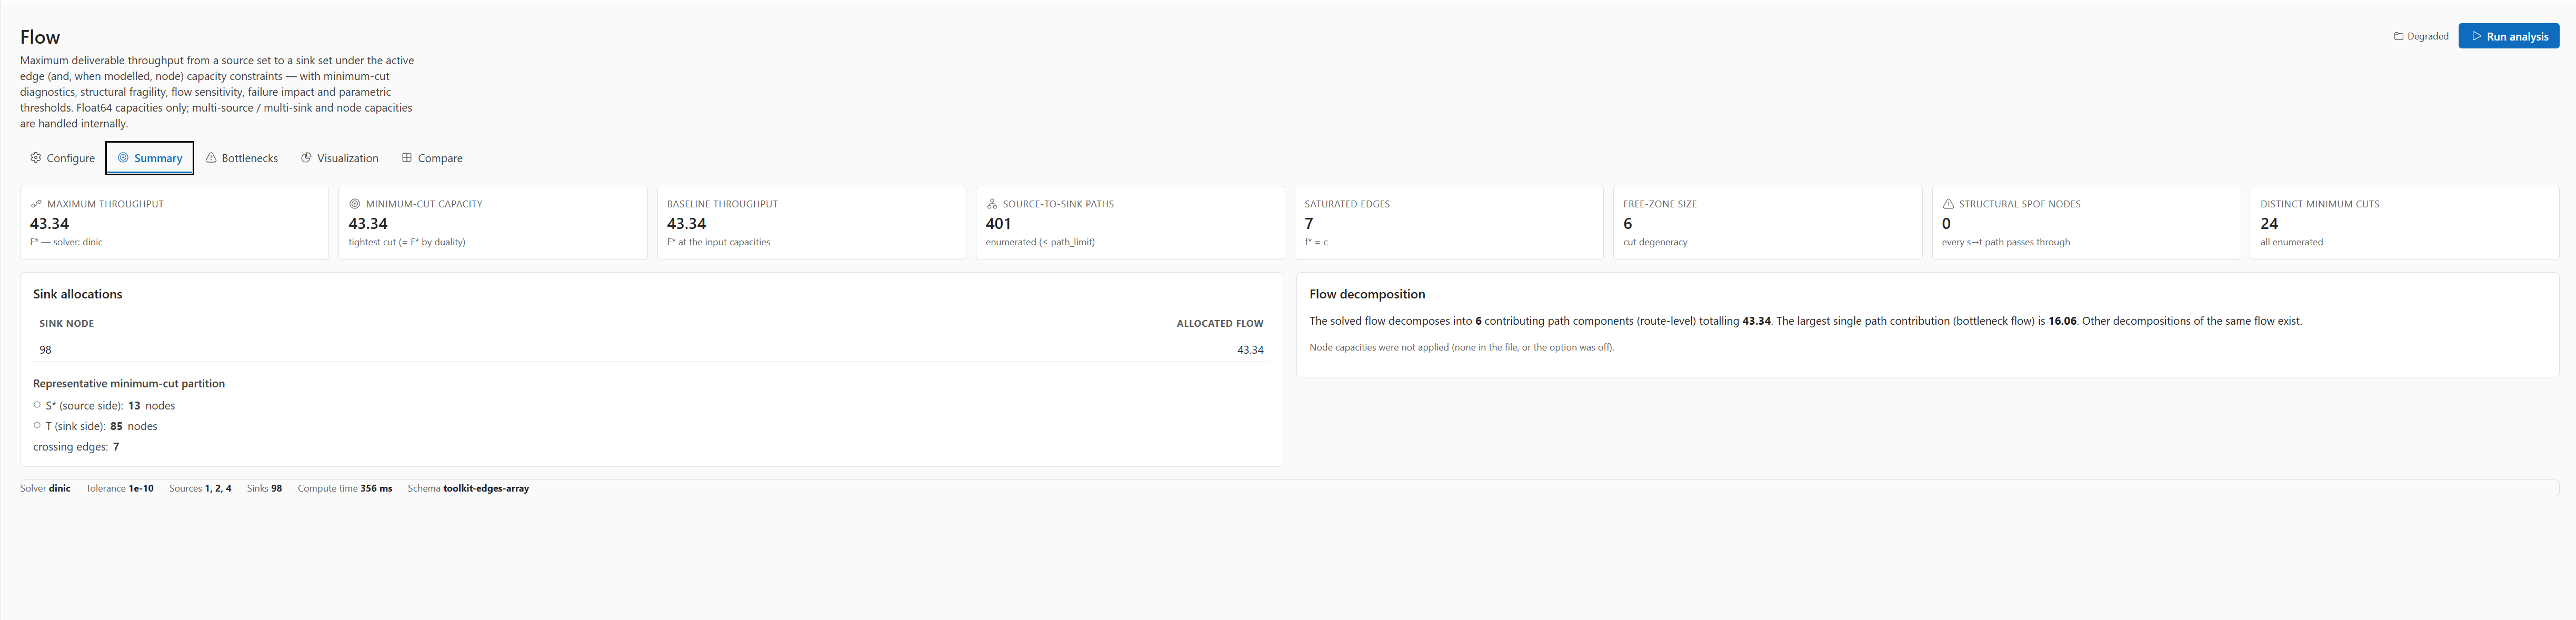
\includegraphics[width=\linewidth]{fig09_flow_degraded.png}
  \caption{Flow summary, degraded scenario: 43.3 litres per second, 6.4 per cent of demand,
  with seven saturated edges, a free zone of six nodes and 24 minimum cuts.}
  \label{fig:e2e-degraded}
\end{figure}

\section{Schedule}
\label{sec:e2e-schedule}

The restoration programme completes in 1,773.3 hours, about 74 days, along a chain of 28
activities that runs from the river reservoir through the trunk main and the eastern loop
to junction 69 (Figure~\ref{fig:e2e-schedule}); 27 further activities are within ten per
cent of the project value. The chain is long because the regulatory holds add 64 hours to
every pipe it passes, and it runs where it does because the trunk main's 12.6-hour flush
falls on it. Under the interval durations the project value lies in $[1{,}418.7, 2{,}128.0]$
hours, the two corners of the input box (Figure~\ref{fig:e2e-schedule-interval}). The exact
floats by the domination split were declined: the 122 non-degenerate interval durations
exceed the fixed screening threshold of Chapter~\ref{ch:critical-path}, so the toolkit
returned the conservative enclosure, tagged as such on the screen, under which no activity
is necessarily critical and 61 are possibly critical. Section~\ref{sec:e2e-findings}
returns to this.

\begin{figure}[htbp]
  \centering
  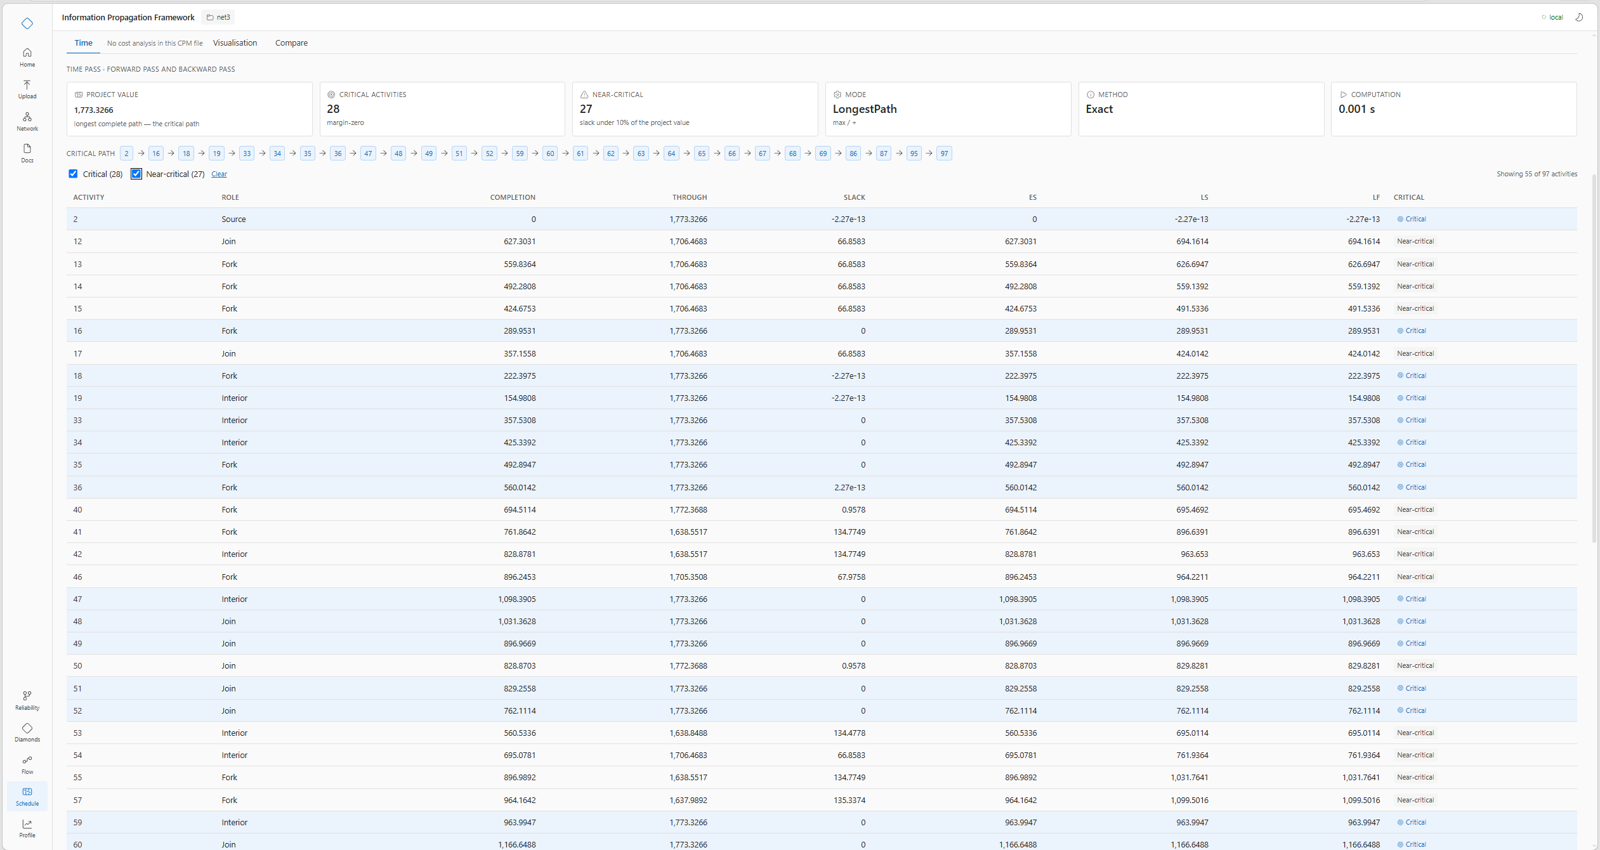
\includegraphics[width=\linewidth]{fig10_schedule_baseline.png}
  \caption{Schedule, baseline, LongestPath: project value 1,773.3 hours, 28 critical and 27
  near-critical activities, with the critical chain and the per-activity schedule
  quantities.}
  \label{fig:e2e-schedule}
\end{figure}

\begin{figure}[htbp]
  \centering
  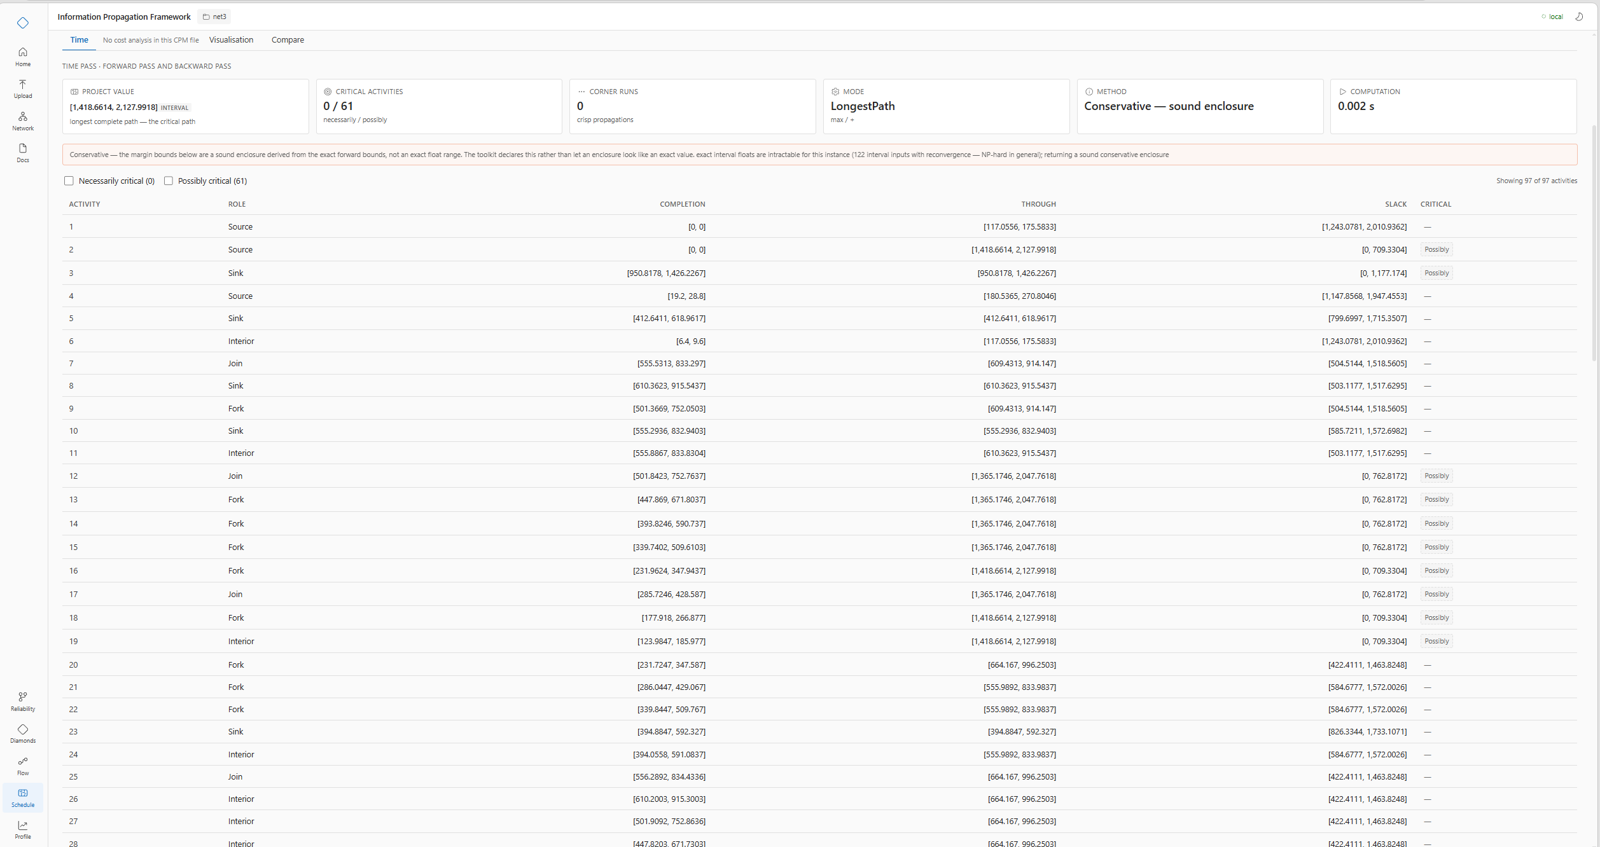
\includegraphics[width=\linewidth]{fig11_schedule_interval.png}
  \caption{Schedule, interval scenario: project value $[1{,}418.7, 2{,}128.0]$ hours. The
  method tag reads conservative enclosure and the banner states why the exact split was
  declined; 0 activities necessarily critical, 61 possibly critical.}
  \label{fig:e2e-schedule-interval}
\end{figure}

The multiplicative mode answers a different question on the same topology: with the
reliability probabilities as the factors, the best single route to each node is the most
reliable route to it. The best route in the network compounds to 0.9928, and the least
reliable best route reaches node 76 at 0.7515 (Figure~\ref{fig:e2e-maxscaling}). Node 76 is
the worst-served node under both interpretations, which is expected, since its low belief
is the product of the same long chain of pipe probabilities that makes its best route
weak; the two analyses agree on where the problem is and differ in what they say about it,
one giving the probability that any route works and the other the reliability of the best
one. The Compare tab (Figure~\ref{fig:e2e-compare}) places the four schedule scenarios side
by side, with the interval row carrying its two criticality counts in separate columns.

\begin{figure}[htbp]
  \centering
  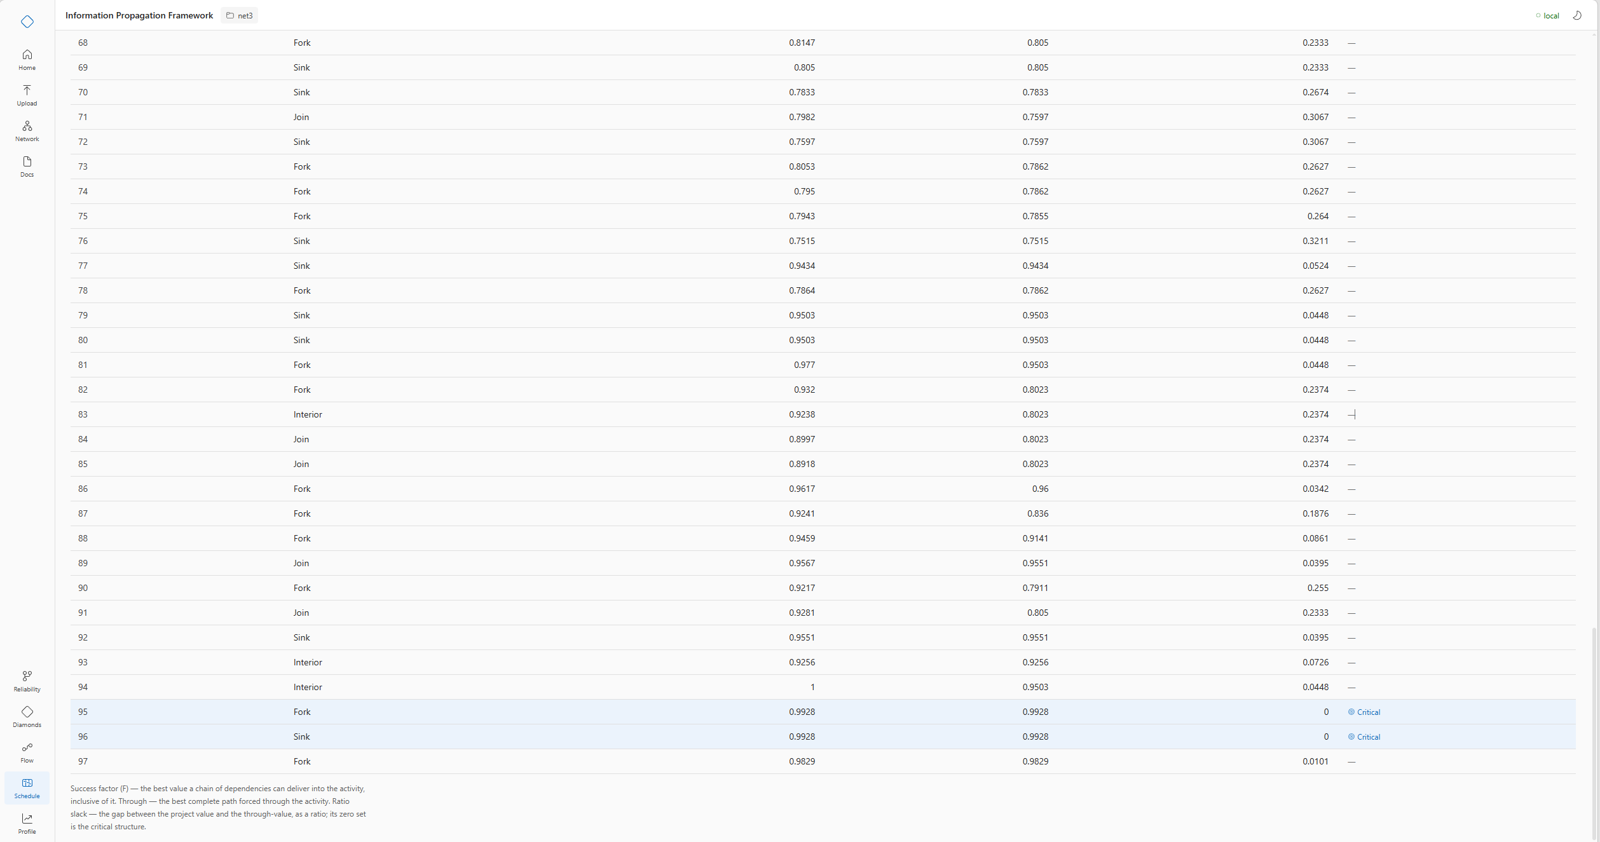
\includegraphics[width=\linewidth]{fig12_schedule_maxscaling.png}
  \caption{Schedule, MaxScaling mode with the reliability probabilities as factors, showing
  the table rows around node 76: the best route in the network compounds to 0.9928 and the
  weakest best route reaches node 76 at 0.7515.}
  \label{fig:e2e-maxscaling}
\end{figure}

\begin{figure}[htbp]
  \centering
  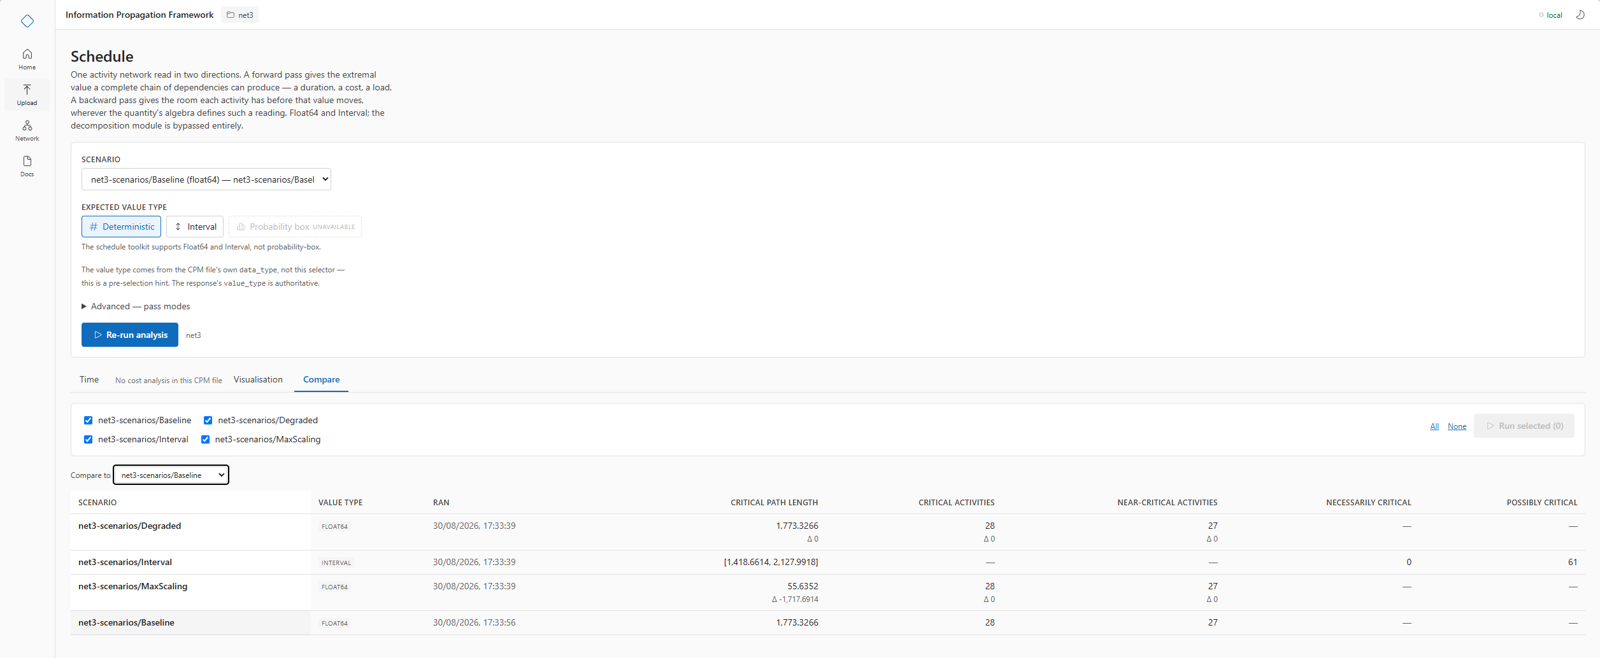
\includegraphics[width=\linewidth]{fig13_schedule_compare.png}
  \caption{The schedule Compare tab across the four scenarios, with the baseline selected
  for differences. The interval row reports necessarily and possibly critical counts
  separately.}
  \label{fig:e2e-compare}
\end{figure}

\section{Two Result Sets on One Drawing}
\label{sec:e2e-profile}

The profile page draws any result set on the network and overlays a second.
Figure~\ref{fig:e2e-profile} draws the edges in every minimum cut of the degraded scenario
against the critical path of the baseline schedule. The baseline cut is not drawn, because
it is the set of demand edges and marks every demand junction. The two sets share three
nodes. One is the super-sink, at which every cut edge ends and, in the edge list with the
super-sink added, the critical path too. Nodes 95 and 97, the ends of the river pump, are
the other two. The pump whose loss leaves 6.4 per cent of the demand served also lies on the chain
that sets the 74 days of restoration, so reinstating it is the step that both analyses
point to. The conditioning set of the reliability analysis, the union across all 307
diamonds, is a third set of 26 nodes, and it too can be drawn.

\begin{figure}[htbp]
  \centering
  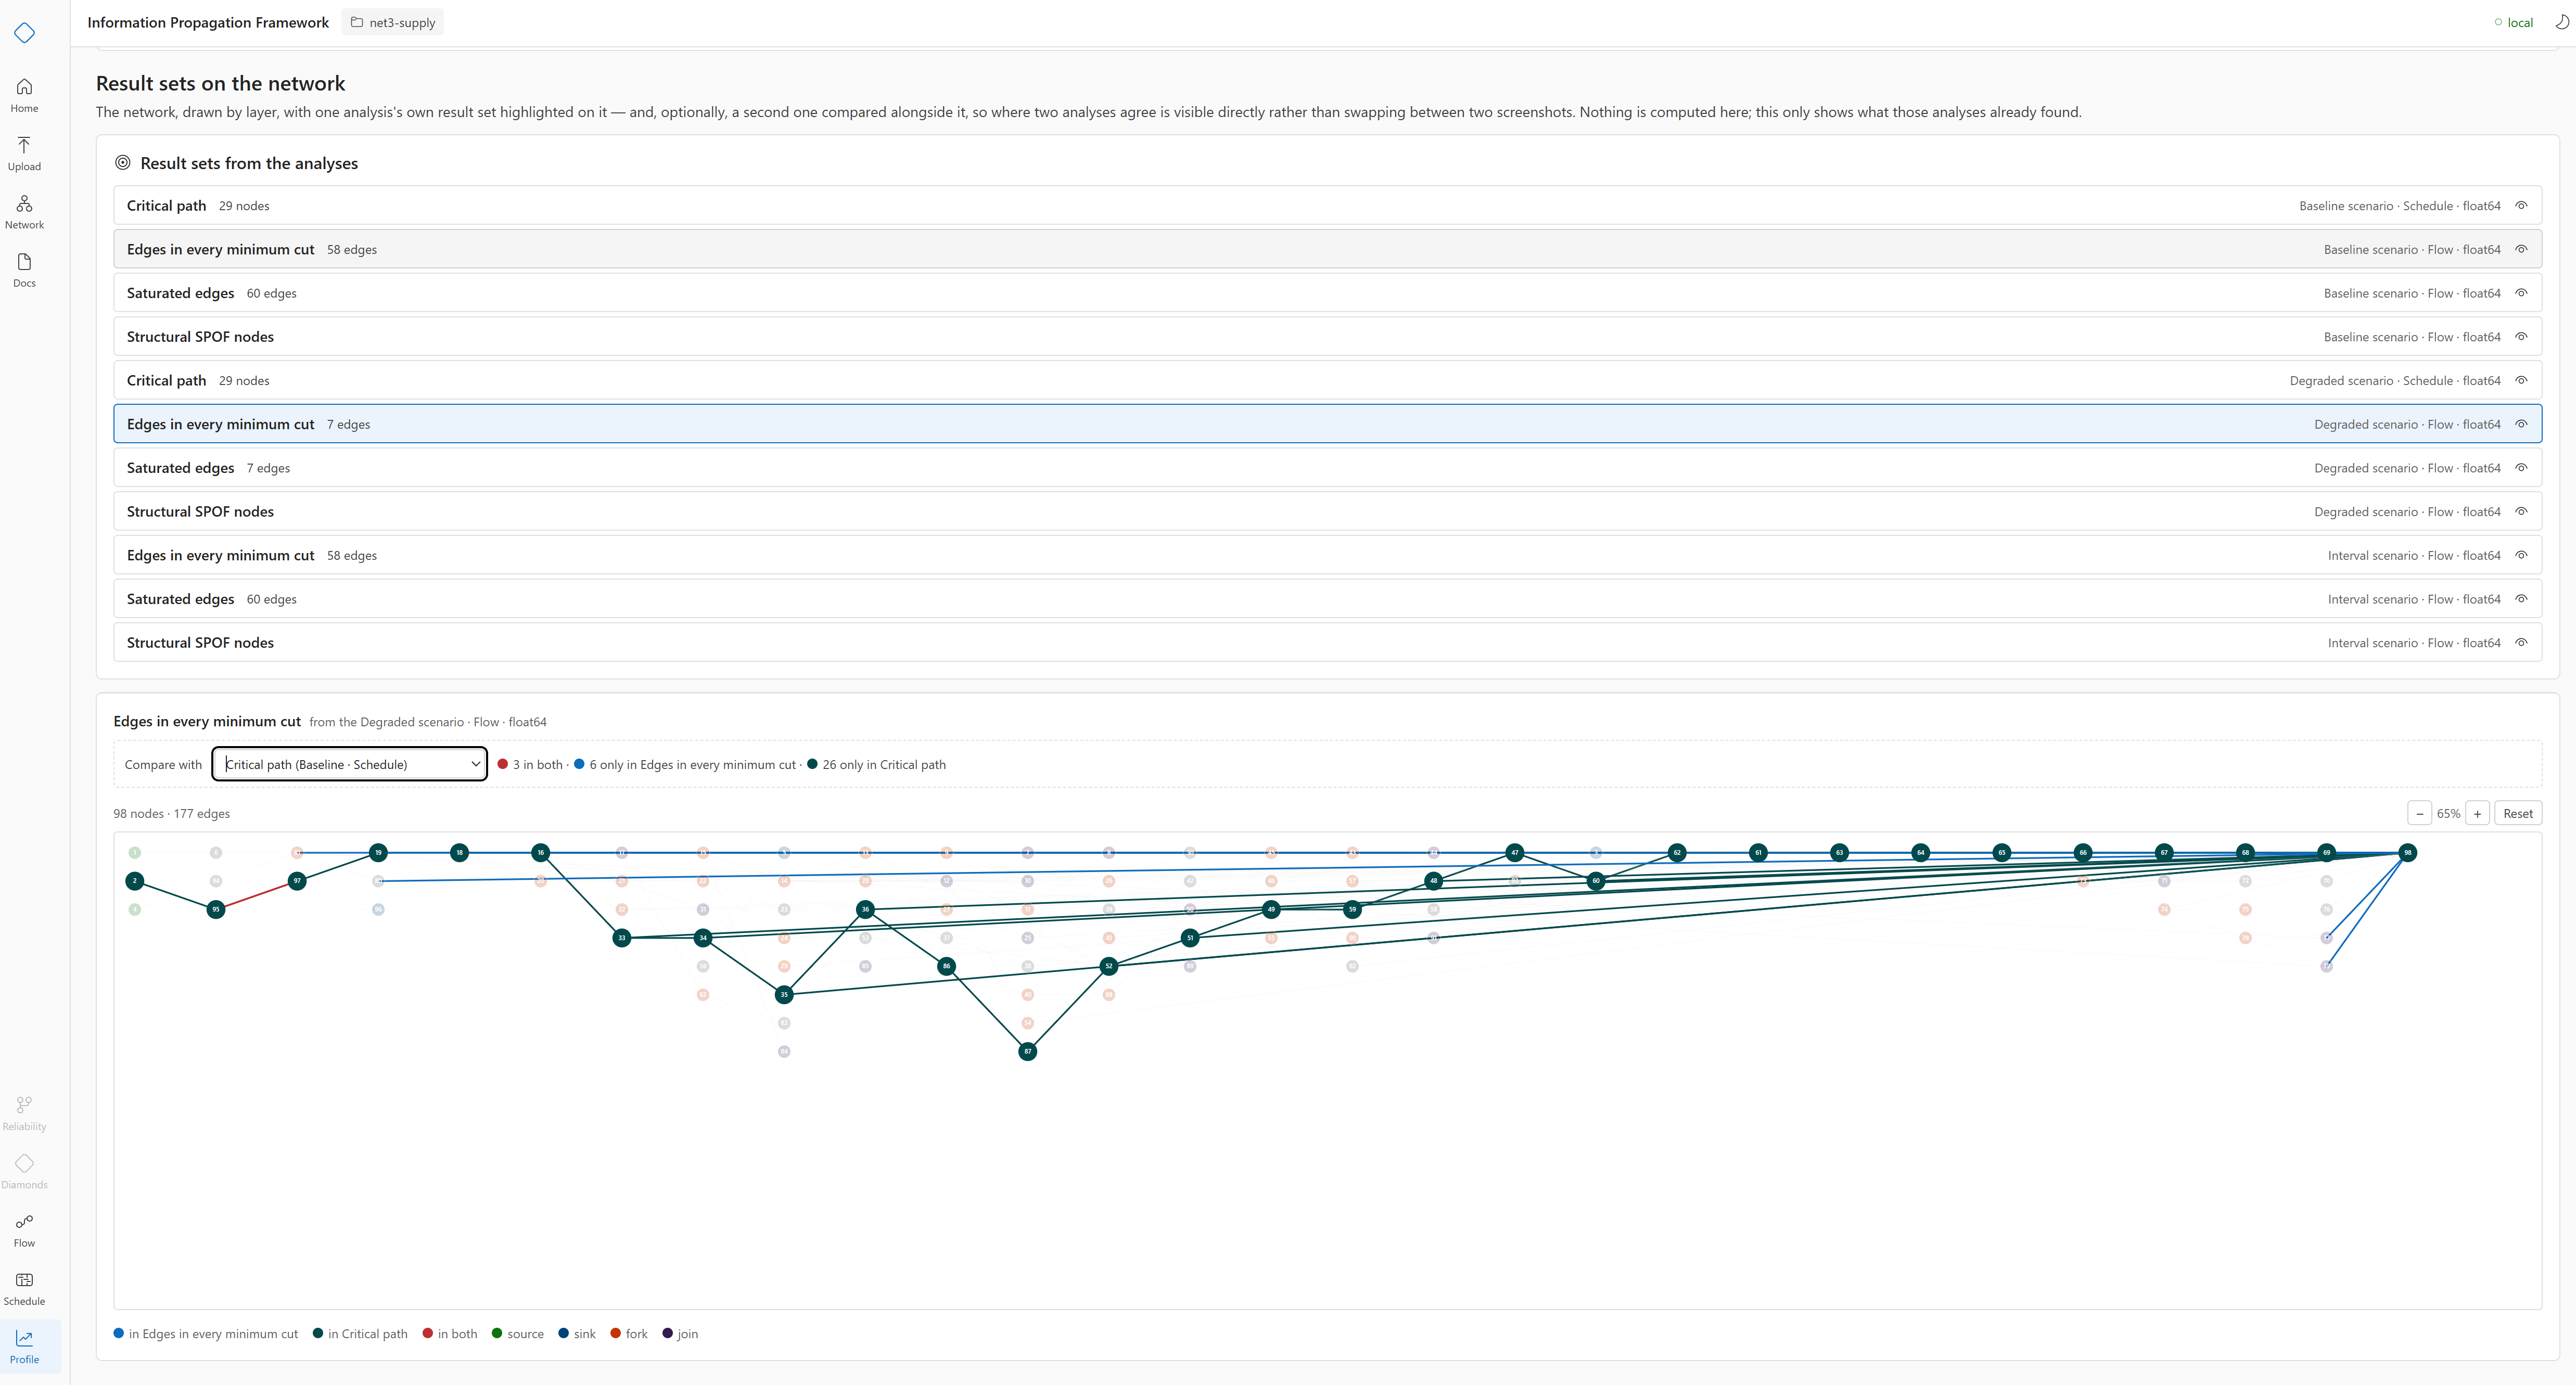
\includegraphics[width=\linewidth]{fig14_profile_overlay.png}
  \caption{The profile page: the edges in every minimum cut of the degraded flow overlaid
  with the critical path of the baseline schedule, on the network drawn by layer. With the
  super-sink in the edge list the critical path has 29 nodes, the 28 activities and the
  super-sink. Three nodes are in both: 95, 97 and the super-sink.}
  \label{fig:e2e-profile}
\end{figure}

\section{What the Run Showed About the Framework}
\label{sec:e2e-findings}

Three toolkits ran on one converted network. The reliability and schedule analyses read the
graph object of the converted edge list, and the capacity analysis read the same edge list
with the super-sink of Section~\ref{sec:e2e-inputs} added, as the IEEE case of
Chapter~\ref{ch:capacity-toolkit} does. Each toolkit added its own input file, and none of
the three required a change to the others' files. The whole sequence, including a second
scenario for each toolkit, took under a minute of computation in a warm process: 4.6, 4.1
and 2.1 seconds for the three baseline runs.

However, two boundaries of the framework were reached on this network, and both are the
boundaries the earlier chapters located. The probability-box form was not run, because the network's
conditioning cost is past the point Chapter~\ref{ch:probability-toolkit} identified as
practical. The exact interval floats were declined, because 122 interval durations exceed
the screening threshold of Chapter~\ref{ch:critical-path}; the split was not priced, and
on a network whose bypass sets might have been small that is a limitation of the screen, which
Chapter~\ref{ch:conclusions} lists as future work. The PSPLIB instance of
Chapter~\ref{ch:critical-path} never approached either boundary. A real network of
moderate size reached both.

Three errors were found and fixed in the course of the run, and they are added to the
record of Chapter~\ref{ch:julia-package}. The unbounded reservoir capacities were the first
inputs to produce an infinite value in an analysis result, and the server's serialiser
refused it; non-finite values are now converted to string tokens at the response boundary.
The interface then rendered that token as not-a-number in one column, which was a second
error, since an unbounded marginal range is a finding. In addition, the schedule
Compare table reported the interval scenario's two criticality counts as a single number,
zero, which collapsed a value form in the way the rules of Chapter~\ref{ch:front-end}
forbid. Each was found because a real network exercised a path the corpus had not, which
is the pattern of every error in Chapter~\ref{ch:julia-package}'s list.

\section{Summary}
\label{sec:e2e-summary}

A public water distribution network was oriented by its own hydraulics, converted once, and
analysed under the three interpretations of Chapter~\ref{ch:system-model}.
Supply reaches its worst-served junction with probability 0.81 at the stated values and
with a certified range of $[0.35, 0.99]$ under five per cent input uncertainty; the network
delivers its whole demand of 680 litres per second, and 43 with the larger pump out, when
only the junctions downstream of the lake pump and the source tank can be served; and its
restoration takes 74 days along a 28-activity chain, between 59 and 89 days under twenty
per cent duration uncertainty. The river pump lies on both the degraded minimum cut and the
restoration critical chain. The run reached two boundaries the earlier chapters had located
and found three implementation errors, each recorded.

\ifdefined\maindoc
\else
\printbibliography
\end{document}
\fi